% pyair2stream: journal article outline.
%
% Structure only. The text is yours to write. Each \prompt{...} says what a
% paragraph should do and points to its evidence in the repository; each
% \fact{...} is a number taken from the repository (validation/REPORT.md, run
% of 2026-10-10, pyair2stream 0.5.1). Rerun the validation suite on the release
% you submit and update every \fact before submission.
%
% Build:  cd paper && latexmk -pdf main.tex      (or pdflatex, bibtex, pdflatex x2)
% Hide the prompts: change \drafttrue to \draftfalse.
%
% Written in plain `article` so it builds anywhere. For Geoscientific Model
% Development, move the text into Copernicus's template (copernicus.cls); the
% section order already follows GMD's model description papers, including the
% required "Code and data availability" section.

\documentclass[11pt,a4paper]{article}

\usepackage[T1]{fontenc}
\usepackage[utf8]{inputenc}
\usepackage{lmodern}
\usepackage[margin=25mm]{geometry}
\usepackage{amsmath,amssymb}
\usepackage{graphicx}
\usepackage{booktabs,tabularx,multirow}
\usepackage{siunitx}
\usepackage[round,authoryear]{natbib}
\usepackage{xcolor}
\usepackage[colorlinks=true,linkcolor=blue!50!black,citecolor=blue!50!black,urlcolor=blue!50!black]{hyperref}
\usepackage{lineno}

\graphicspath{{../validation/figures/}{../docs/figures/}{../examples/}}
\sisetup{range-phrase = \text{--}, range-units = single}

% ---------------------------------------------------------------- draft notes
\newif\ifdraft
\drafttrue
\ifdraft
  \newcommand{\prompt}[1]{\par\noindent\fcolorbox{orange!70!black}{orange!8}{%
    \parbox{\dimexpr\linewidth-2\fboxsep-2\fboxrule}{\small\sffamily\textbf{Write:} #1}}\par\medskip}
  \newcommand{\fact}[1]{\textcolor{teal!70!black}{#1}}
  \linenumbers
\else
  \newcommand{\prompt}[1]{}
  \newcommand{\fact}[1]{#1}
\fi
\newcommand{\pkg}{\texttt{pyair2stream}}
\newcommand{\aas}{\texttt{air2stream}}
\newcommand{\repo}[1]{\texttt{#1}}   % a file in the repository

% Software version and archive: fill in at release.
\newcommand{\version}{0.5.1}
\newcommand{\softwaredoi}{10.5281/zenodo.XXXXXXX}

\title{\pkg{} v\version: an open, tested Python implementation of the
\aas{} river temperature model, with uncertainty quantification and
cross-validation}
% GMD requires the model name and version number in the title.

\author{Luke Fullard\thanks{Affiliation, address. Correspondence: email.}
% \and Co-authors
}
\date{}

\begin{document}
\maketitle

% =========================================================================
\begin{abstract}
\prompt{About 200--250 words, five or six sentences:
(1) why daily river temperature matters, and why it must often be predicted
from air temperature and discharge alone;
(2) \aas{} \citep{toffolon2015} and its standing (widely used; Fortran
original);
(3) what \pkg{} is: a Python implementation that reproduces the Fortran
to \fact{\SI{5e-6}{\celsius}}, plus what it adds (uncertainty by DE-MCMC with an
autocorrelated error model, prediction intervals and paired scenarios,
year-by-year cross-validation, conformal margins, gap-tolerant runs,
input and stability checks);
(4) how it was tested: \fact{402} automated tests and a 19-check validation
suite with criteria stated in advance, against the Fortran, three published
studies and 26 rivers in Switzerland and British Columbia;
(5) the main findings, including the failures (intervals hold at
\fact{87--90\%} for a stated 90\% on held-out data; too narrow on the hottest
days and on some British Columbia rivers, which the optional conformal
margins correct; one published calibration found to have its seasonal
cycle ten months out of phase);
(6) availability and licence.}
\end{abstract}

\noindent\textbf{Keywords:} river water temperature; air2stream; hybrid
model; uncertainty quantification; Markov chain Monte Carlo;
cross-validation; conformal prediction; reproducibility; open-source software

% =========================================================================
\section{Introduction}
\label{sec:intro}

\prompt{Why river temperature matters: aquatic ecology (fish thermal
limits), regulation (temperature limits, permits, compliance), and climate
change and abstraction scenarios. Where a decision rests on it, the
prediction must come with an honest range.}

\prompt{The modelling options: process-based energy-balance models (data
hungry), statistical regressions on air temperature (simple, but poor
outside the calibration range), and hybrid models. Introduce \aas{}
\citep{toffolon2015}, its lake counterpart \texttt{air2water}
\citep{piccolroaz2013}, its comparison with statistical approaches
\citep{piccolroaz2016}, and independent evaluations
\citep[e.g.][]{callahan2025}.}

\prompt{The gap this paper fills. The Fortran original
\citep{air2stream_code} gives a best fit only: no parameter or prediction
uncertainty, no cross-validation, few input checks; it assumes a record
starts on 1 January; it is distributed as source and a Windows executable.
Results used in regulation or in court must be reproducible, tested and
carry a stated confidence.}

\prompt{Contributions, as a list:
(i) a verified port of every model version, integrator and objective;
(ii) uncertainty quantification designed for autocorrelated errors;
(iii) year-by-year cross-validation, bias correction of yearly statistics,
and conformal margins;
(iv) scenario comparisons with paired simulations;
(v) a validation suite with stated pass criteria, whose failures are
reported;
(vi) the outline of the paper.}

% =========================================================================
\section{The air2stream model}
\label{sec:model}

\prompt{A short recap for readers who do not know the model; the
original papers carry the derivation. Source:
\repo{docs/METHODS.md} §1--§9.}

\subsection{Governing equation and model versions}
The full eight-parameter model is
\begin{equation}
  \frac{\mathrm{d}T_w}{\mathrm{d}t} = \frac{1}{\theta^{a_4}}
  \left[ a_1 + a_2 T_a - a_3 T_w
  + \theta \left( a_5 + a_6 \cos\!\left(2\pi\left(t - a_7\right)\right) - a_8 T_w \right) \right],
  \label{eq:a2s}
\end{equation}
with $T_w$ the water temperature, $T_a$ the air temperature, $t$ the time of
year as a fraction, and $\theta = Q/\bar{Q}$ the discharge scaled by its
mean over the calibration period (\texttt{Qmedia}).

\prompt{Explain each term in words (METHODS §5), and why $\bar{Q}$ is held at
the calibration value in prediction and scenario runs (METHODS §4).}

\begin{table}[htbp]
  \centering
  \caption{Model versions: the simpler ones fix parameters at zero.}
  \label{tab:versions}
  \begin{tabular}{@{}cllcc@{}}
    \toprule
    Version & Parameters & Right-hand side & Discharge & Seasonal term \\
    \midrule
    3 & $a_1$--$a_3$ & $a_1 + a_2T_a - a_3T_w$ & no & no \\
    4 & $a_1$--$a_4$ & $(a_1 + a_2T_a - a_3T_w)/\theta^{a_4}$ & yes & no \\
    5 & $a_1$--$a_3$, $a_6$, $a_7$ & $a_1 + a_2T_a - a_3T_w + a_6\cos(\cdot)$ & no & yes \\
    7 & all but $a_4$ & Eq.~\eqref{eq:a2s} with $\theta^{a_4}=1$ & yes & yes \\
    8 & $a_1$--$a_8$ & Eq.~\eqref{eq:a2s} & yes & yes \\
    \bottomrule
  \end{tabular}
\end{table}

\subsection{Numerical solution}
\prompt{The daily time step and the five integrators: Crank--Nicolson
(\texttt{CRN}), exponential (\texttt{EXP}), RK4, RK2 and Euler. Stability of
the explicit schemes, and why parameters belong to the scheme they were
calibrated with (METHODS §6; the evidence is V6 and V13).}

\subsection{Objective functions and calibration}
\prompt{NSE \citep{nash1970}, RMSE and KGE \citep{gupta2009}, scored on daily,
weekly or monthly means. The warm-up year (METHODS §3). Optimizers:
differential evolution \citep{storn1997} with L-BFGS-B polishing
\citep{byrd1995} as the default, plus PSO \citep{kennedy1995} and Latin
hypercube as in the Fortran.}

% =========================================================================
\section{Implementation}
\label{sec:implementation}

\subsection{Design and architecture}
\prompt{The software stack: NumPy, SciPy, pandas and matplotlib; the time loop
is compiled with Numba \citep{lam2015}; MCMC uses emcee
\citep{foremanmackey2013}. One settings file (YAML) describes a run, and the
run modes are calibration, DE-MCMC, FORWARD and cross-validation.
Interfaces: the command line, \texttt{pyair2stream.run} and the
\texttt{pyair2stream.Model} workflow (calibrate, check, predict). Each run
writes a summary (\texttt{summary.md}/\texttt{.html}) and its settings, so
it can be audited and repeated. A figure could show the workflow (data,
calibration, check, prediction, scenario).}

% \begin{figure}[htbp]
%   \centering
%   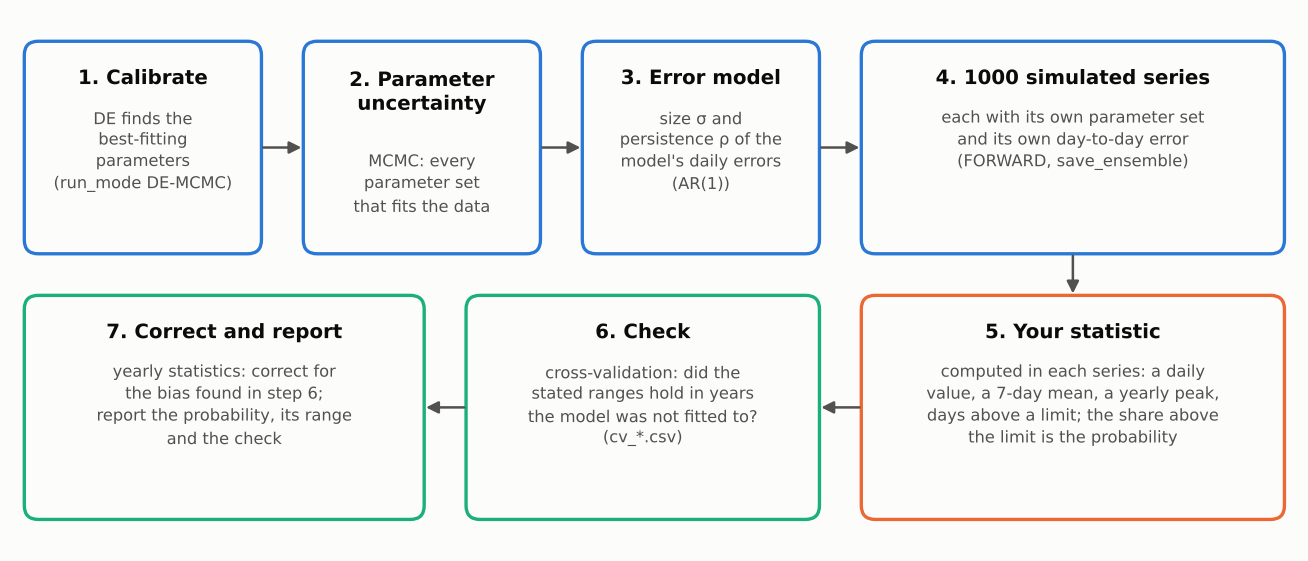
\includegraphics[width=\linewidth]{U01_pipeline.png}
%   \caption{From data to a statement with a stated confidence: the steps \pkg{} runs.}
%   \label{fig:workflow}
% \end{figure}

\subsection{Correspondence with the Fortran original, and deliberate differences}
\prompt{Everything the Fortran computes is reproduced (Sect.~\ref{sec:v-fortran}).
Where the two differ, \pkg{} differs on purpose, because the Fortran was wrong
or silent; Table~\ref{tab:differences} lists each case. Source:
\repo{docs/METHODS.md} §17.}

\begin{table}[htbp]
  \centering
  \caption{Deliberate differences from the Fortran original
  (\repo{docs/METHODS.md} §17). Each is covered by a test.}
  \label{tab:differences}
  \small
  \begin{tabularx}{\linewidth}{@{}lXX@{}}
    \toprule
    Topic & Fortran & \pkg{} \\
    \midrule
    Seasonal phase & from the row number; a record is assumed to start on 1~January, unchecked
                   & from each row's date; a record may start on any date \\
    PSO global best & taken from a score array that is still zero, so always the first particle
                    & the best initial particle \\
    PSO stopping & a test that can never be met & tolerance $10^{-4}$ \\
    \texttt{Qmedia} & recomputed from each file, including days the model cannot simulate
                    & fixed at the calibration value; zero-flow days excluded where they cannot be simulated \\
    Weekly/monthly scoring & out-of-range index in a partial last block; division by zero when \texttt{prc}=0
                           & a block without data is never scored; \texttt{prc} applies to the calendar length \\
    Input checks & none: runs on silently & missing, implausible or non-positive inputs; unused parameters; stability and divergence \\
    Defaults & --- & \texttt{CRN} integrator; DE with L-BFGS-B \\
    \bottomrule
  \end{tabularx}
\end{table}

\subsection{Data handling}
\prompt{Input checks (METHODS §2 and §15). Gap-tolerant mode: segments are
started at rest (METHODS §10). Non-standard calendars (365-day, 360-day)
for climate-model inputs. Zero discharge and \texttt{min\_theta\_floor}.}

% =========================================================================
\section{Uncertainty quantification}
\label{sec:uq}

\prompt{The core methodological contribution. Present it as a chain: error
model, then parameter uncertainty, then prediction intervals, then a check on
held-out years, then a correction where the check fails. Source:
\repo{docs/METHODS.md} §11--§13 and \repo{docs/UNCERTAINTY.md}.}

\subsection{Error model and likelihood}
\prompt{Model errors persist from day to day, so treating them as independent
understates the uncertainty. Describe the AR(1) error model and the effective
number of observations $n_\mathrm{eff} = n/F$ \citep{bayley1946}, with $F$
summed over the pairs of scored days, so gaps are handled. Give the
log-likelihood $-\tfrac{n_\mathrm{eff}}{2}\ln(\mathrm{SSE}/n)$; its maximum
is the least-squares fit. Explain why $\rho$ is estimated on a weekly scale
rather than from consecutive days (evidence: V4, V18;
\citealp{mcinerney2020}). Compare the exact AR(1) likelihood and the
independent-error likelihood, and say why neither is the default
\citep{evin2014}.}

\begin{equation}
  \log L(\mathbf{a}) = -\frac{n_\mathrm{eff}}{2}\,\ln\!\frac{\mathrm{SSE}(\mathbf{a})}{n},
  \qquad
  F = 1 + \frac{2}{n}\sum_{i<j} \rho^{\lvert t_i - t_j\rvert}.
  \label{eq:likelihood}
\end{equation}

\subsection{Parameter uncertainty by DE-MCMC}
\prompt{The prior is uniform within the bounds. Sampling starts from the DE
best fit, with the affine-invariant ensemble sampler
\citep{goodman2010,foremanmackey2013}. Convergence is judged by the
autocorrelation time and split-$\hat{R}$ \citep{gelman2013}. Jackknife
parameter intervals come from cross-validation \citep{kunsch1989}.}

\subsection{Prediction intervals and paired scenarios}
\prompt{A FORWARD run draws parameter sets from the chain and adds AR(1) noise
\citep{box2015}, giving an ensemble of series. Intervals for days, 7-day and
30-day means, and yearly statistics (highest daily mean, highest 7-day mean,
days above a threshold) come from the ensemble. Paired scenarios reuse the
same parameter draws and noise, so the uncertainty common to both cancels in
their difference (METHODS §13). Use example 04 (abstraction) as the
illustration.}

\subsection{Cross-validation, bias correction and conformal margins}
\prompt{Leave one year out \citep{stone1974,klemes1986}: the hidden year keeps
its air temperature and discharge (justified by V12;
\citealp{burman1994}). From the held-out years, report the interval coverage
and the bias of each yearly statistic, corrected in the manner of model output
statistics \citep{glahn1972}. Optional conformal margins widen an interval by
the amount held-out years fell outside it
\citep{vovk2005,lei2018,romano2019}; describe the exchangeability caveat
\citep{oliveira2024}. Judge probabilities by the Brier score
\citep{brier1950} and the PIT \citep{gneiting2007}.}

\subsection{Sensitivity analysis}
\prompt{One sentence or two: a local, one-at-a-time index (METHODS §14), and
its limits.}

% =========================================================================
\section{Verification and validation}
\label{sec:validation}

\prompt{Separate verification (is the code right?) from validation (is the
method fit for purpose?). Every check states its question, method and pass
criterion before its result, and all are reported, including those that fail.
Reproducibility: seeded, with software versions recorded. Source:
\repo{validation/README.md} and \repo{validation/REPORT.md}.
Table~\ref{tab:validation} is the map of this section.}

\begin{table}[htbp]
  \centering
  \caption{The validation suite (\repo{validation/REPORT.md}; run of
  2026-10-10, \pkg{} \version). \fact{Update the results for the release submitted.}}
  \label{tab:validation}
  \small
  \begin{tabularx}{\linewidth}{@{}llXc@{}}
    \toprule
    & Check & Question & Result \\
    \midrule
    \multirow{2}{*}{Verification}
      & V1  & Same results as the Fortran (all versions, integrators, objectives; with gaps) & \fact{pass} \\
      & V6  & Numerical accuracy; warnings on unstable runs & \fact{pass} \\
    \midrule
    \multirow{3}{*}{Published results}
      & V13 & Toffolon and Piccolroaz (2015) & \fact{pass} \\
      & V2  & Piccolroaz et al.\ (2016): 3 Swiss rivers, every version & \fact{pass} \\
      & V15 & Callahan and Moore (2025): 23 rivers in British Columbia & \fact{pass} \\
    \midrule
    \multirow{3}{*}{Known truth}
      & V3  & Calibration recovers known parameters & \fact{pass} \\
      & V7  & Gaps do not bias the result & \fact{pass} \\
      & V8  & Workflow and scenario tools are exact & \fact{pass} \\
    \midrule
    \multirow{4}{*}{Prediction}
      & V5  & Real rivers, years not calibrated on & \fact{fail} \\
      & V10 & Warmer or lower-flow years than calibrated on & \fact{fail} \\
      & V16 & Record length needed & \fact{pass} \\
      & V17 & Better than regression on air temperature? & \fact{pass} \\
    \midrule
    \multirow{7}{*}{Uncertainty}
      & V4  & Intervals calibrated (synthetic data) & \fact{fail} \\
      & V9  & Probabilities of exceeding a limit & \fact{fail} \\
      & V11 & Cross-validated correction of yearly statistics & \fact{pass} \\
      & V12 & Cross-validation design & \fact{pass} \\
      & V14 & Intervals on the hottest days & \fact{fail} \\
      & V18 & Intervals on independent rivers & \fact{fail} \\
      & V19 & Conformal margins on 26 rivers & \fact{pass} \\
    \bottomrule
  \end{tabularx}
\end{table}

\subsection{Software testing}
\prompt{\fact{402} automated tests (unit, regression and documentation-link
tests). Golden tests compile the Fortran and compare outputs. Continuous
integration runs them on several Python versions and against the locked
dependencies (\repo{.github/workflows/tests.yml}).}

\subsection{Agreement with the Fortran}
\label{sec:v-fortran}
\prompt{V1: \fact{all 20 version $\times$ integrator cases agree within
\SI{5e-6}{\celsius}}, the last digit the Fortran prints; \fact{99}
scoring combinations agree, with and without gaps. V6: the schemes' error
against the exact solution.}

\begin{figure}[htbp]
  \centering
  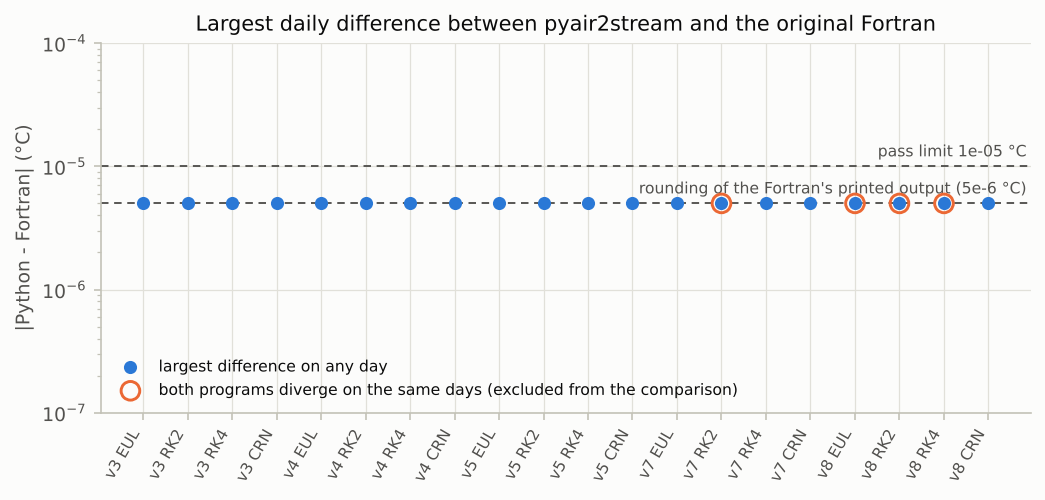
\includegraphics[width=0.8\linewidth]{V1_max_difference.png}
  \caption{Largest difference from the Fortran original, by model version
  and integrator (V1).}
  \label{fig:v1}
\end{figure}

\subsection{Reproducing published results}
\prompt{V13 (2015 paper): reproduced with RK4, not with CRN, so parameters
belong to their integrator. V2 (2016 paper): \fact{all 30 published RMSE values
within \SI{0.0005}{\celsius}}. V15 (British Columbia): \fact{45 of 46} series
reproduced day by day; the 46th has its record starting on 1~November, so
the original's row-based seasonal phase put it ten months out of phase. That
is a concrete case of a silent error that a date-based implementation
prevents; describe it with care and respect for the original authors.}

% \begin{figure}[htbp]
%   \centering
%   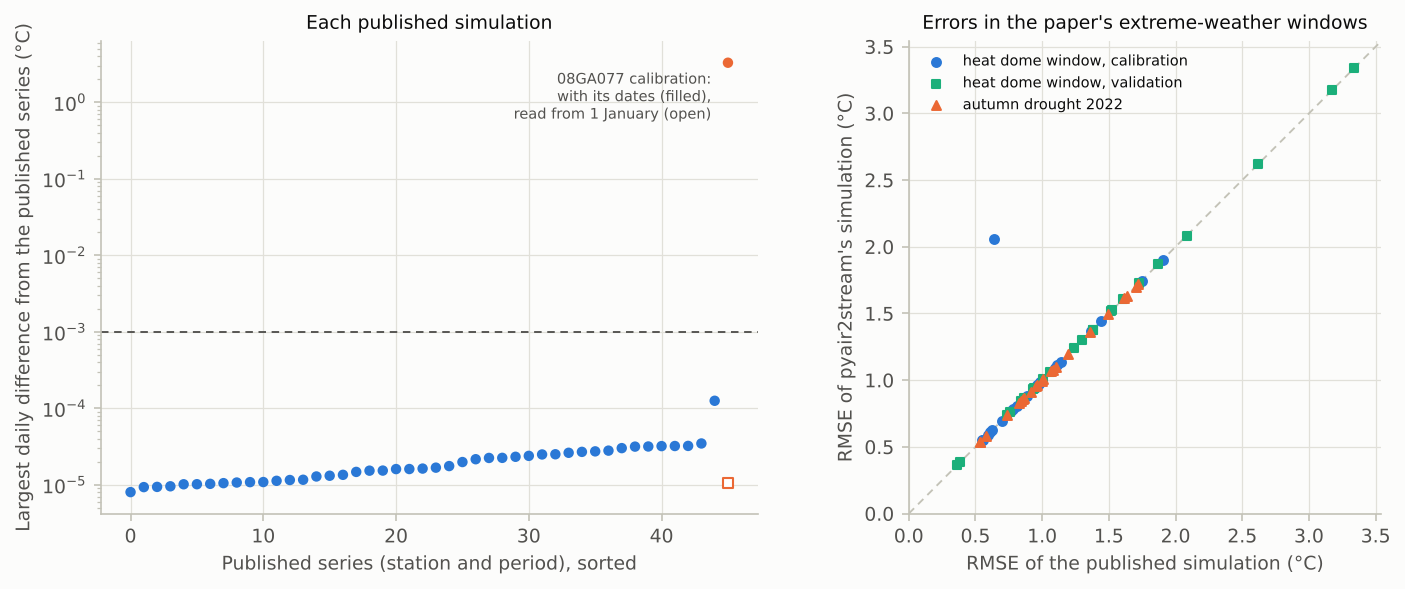
\includegraphics[width=\linewidth]{V15_british_columbia.png}
%   \caption{Published and recomputed simulations, 23 rivers in British Columbia (V15).}
%   \label{fig:v15}
% \end{figure}

\subsection{Recovery of a known truth}
\prompt{V3, V7 and V8, in a short paragraph each, or one paragraph and a
table.}

\subsection{Predictive performance}
\prompt{V5: against simple alternatives on held-out years. V17: version 8
beats every regression on \fact{3 of 3} Swiss and \fact{20 of 23} British
Columbia rivers (median daily RMSE \fact{0.74 against \SI{0.89}{\celsius}};
\fact{0.96 against \SI{1.17}{\celsius}}). V10: extrapolation to the warmest
and lowest-flow years. V16: \fact{3 or more years} of record are close to
the whole record.}

\subsection{Calibration of the uncertainty}
\prompt{The honest heart of the paper. Synthetic data (V4): stated levels are
met to within \fact{3.2} points. Real rivers (V5, V18): the 90\% intervals
hold \fact{85--90\%} of the time; on the hottest days (V14) and some British
Columbia rivers, they are too narrow. Cross-validation corrects yearly
statistics (V11), and conformal margins correct the intervals (V19:
British Columbia 30-day means \fact{84.8\% $\to$ 92.1\%}, without making
the Swiss intervals too wide). Say what each failure means for a user.}

\begin{figure}[htbp]
  \centering
  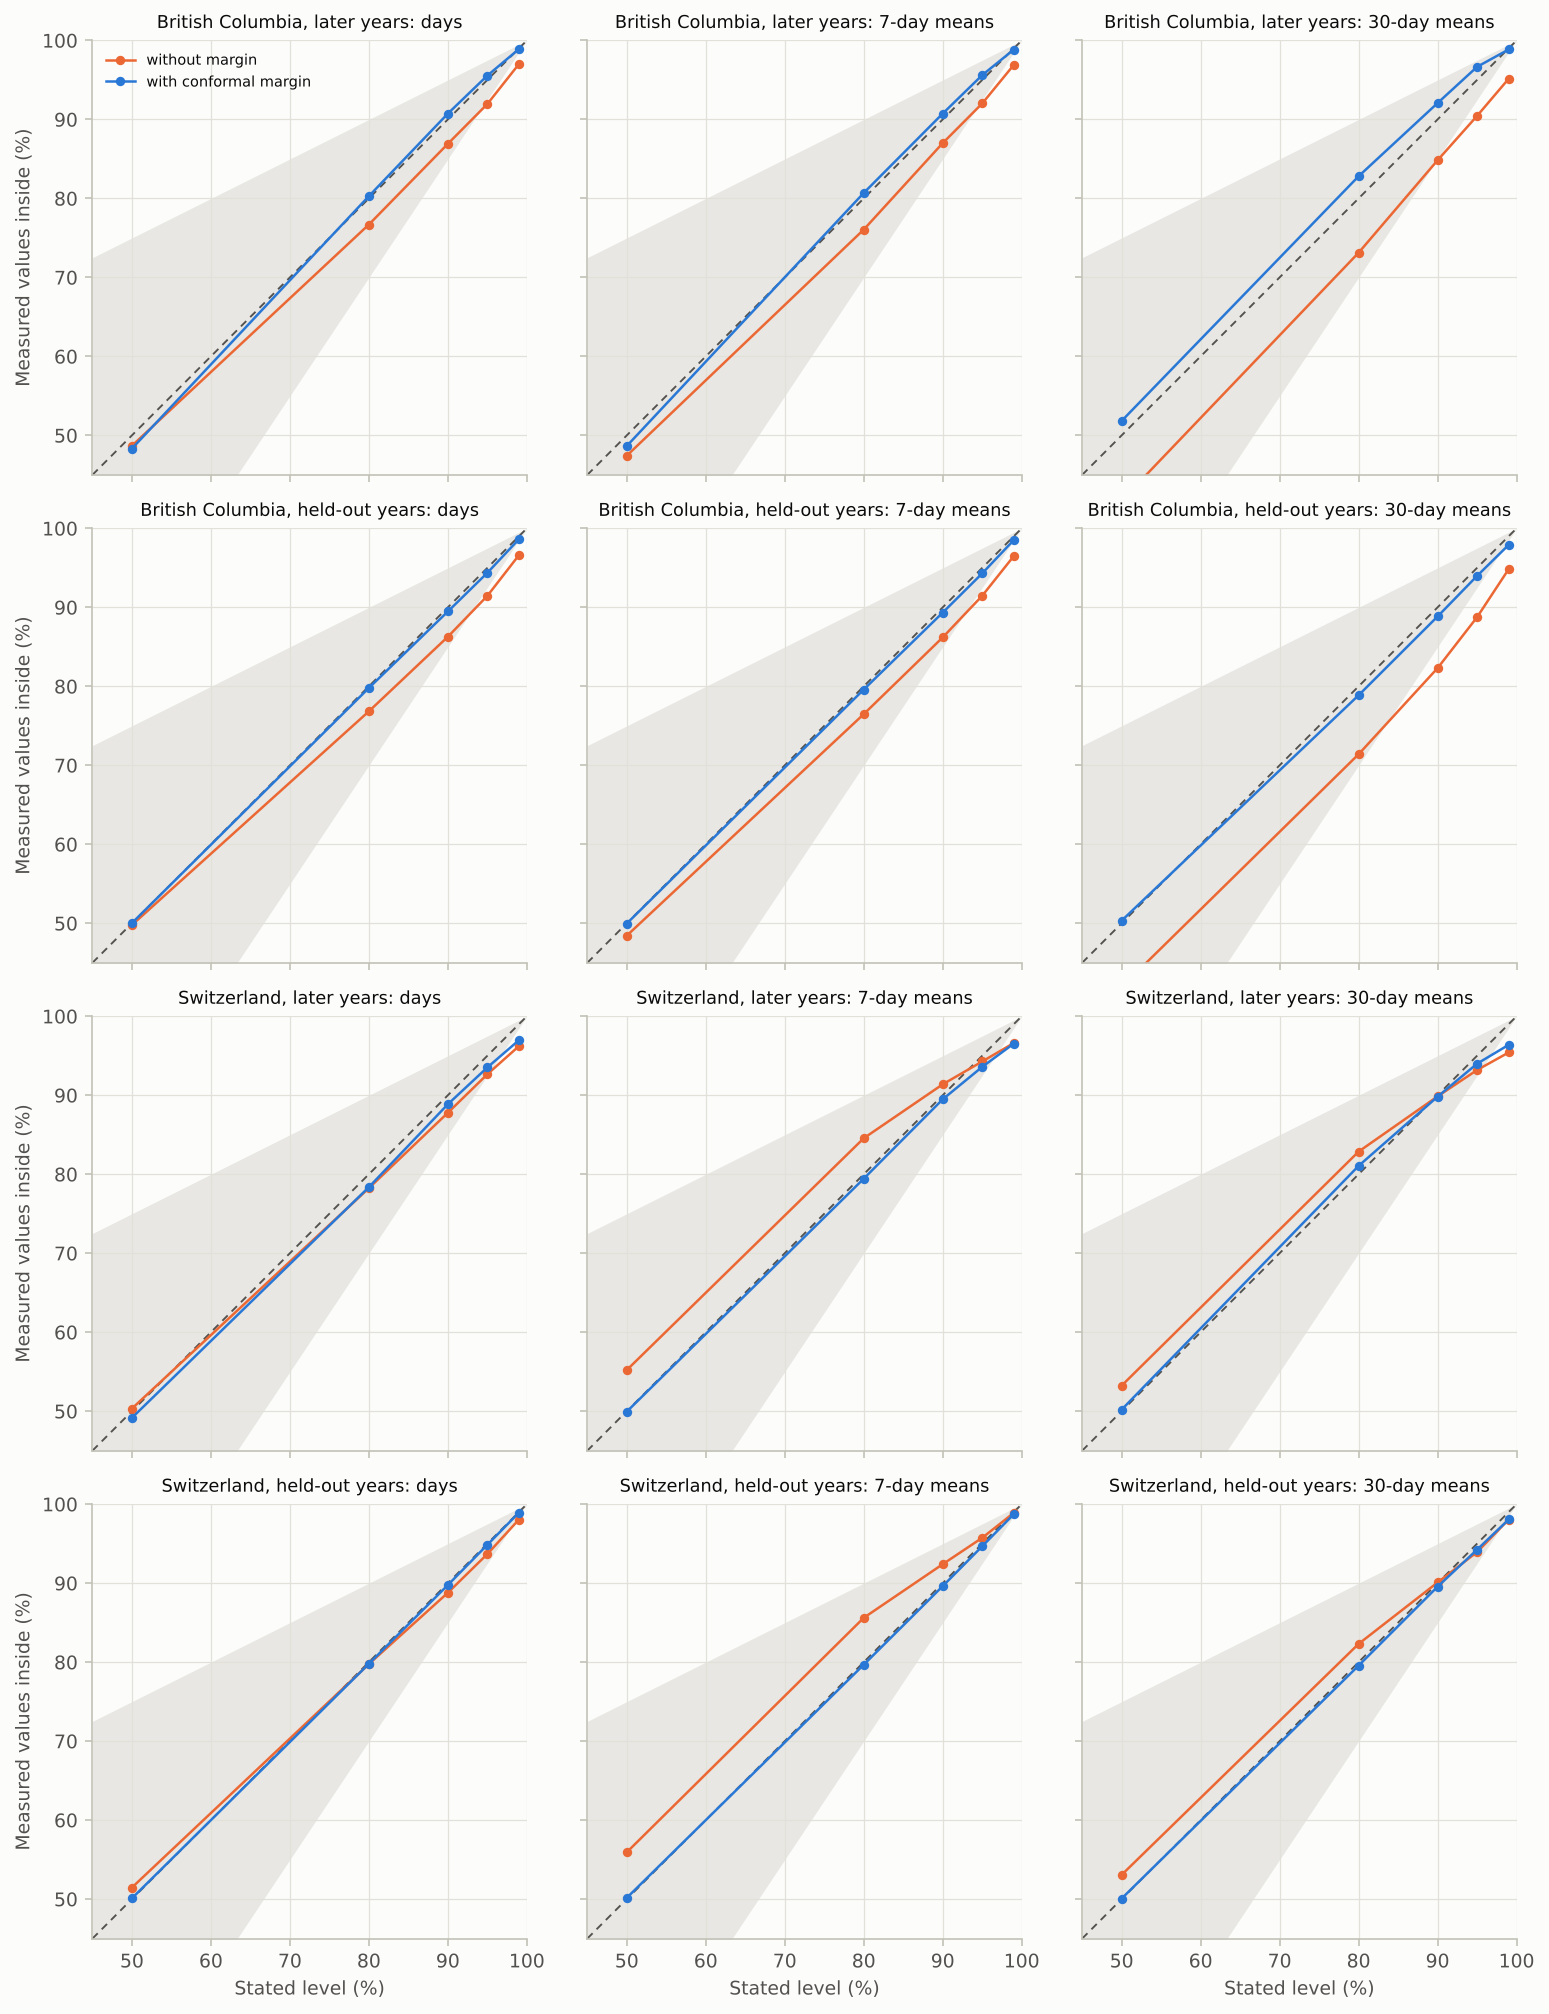
\includegraphics[width=0.8\linewidth]{V19_levels.png}
  \caption{Share of measurements inside the intervals at each stated level,
  without and with conformal margins (V19).}
  \label{fig:v19}
\end{figure}

% =========================================================================
\section{Example application: a compliance question}
\label{sec:example}

\prompt{One worked example from data to a statement. Example 03 asks how likely
it is that the 7-day mean of the Mentue exceeded \SI{20}{\celsius} in
2010--2012. Uncorrected and corrected probabilities: \fact{0.92 / 0.54, 0.77 /
0.35, 0.53 / 0.15}; the Brier score falls from \fact{0.29 to 0.12}
(\repo{examples/03\_compliance/README.md}; \repo{docs/UNCERTAINTY.md}
§16). Optionally, add example 08 (air $+2\,^\circ$C, 20\% less summer flow) to
show paired scenarios. Show the three \texttt{Model} calls (listing below).}

\begin{verbatim}
import pyair2stream
m = pyair2stream.Model("settings.yaml")
m.calibrate()                                   # DE-MCMC
m.predict("2010-2012.csv", name="prediction")   # 1,000 series
m.check()                                       # leave-one-year-out
\end{verbatim}

% \begin{figure}[htbp]
%   \centering
%   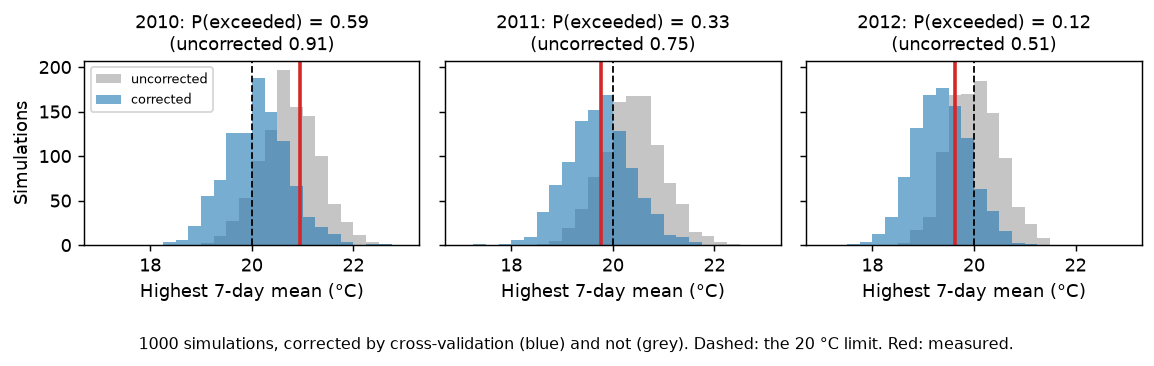
\includegraphics[width=\linewidth]{03_compliance/figures/peak_7day_mean.png}
%   \caption{Highest 7-day mean of each year: predicted range, corrected range and measurement.}
%   \label{fig:example}
% \end{figure}

% =========================================================================
\section{Discussion}
\label{sec:discussion}

\prompt{Limitations: a lumped model at one station; stationarity of the
parameters under climate change and extrapolation (V10); intervals on the
hottest days (V14); the exchangeability assumption behind the conformal
margins; dependence on the prior bounds; the local nature of the sensitivity
index.}

\prompt{Use in regulation and in court: what makes a result defensible
(stated criteria, held-out checks, recorded settings and versions, reruns
that give the same numbers), and what a report should state
(\repo{docs/PUBLISHED\_RESULTS.md}, ``What a publication should state'';
USER\_GUIDE §14).}

\prompt{Relation to the original: an independent port, not maintained or
endorsed by the original authors; the scientific credit for the model is
theirs.}

% =========================================================================
\section{Conclusions}
\label{sec:conclusions}

\prompt{Three to five sentences: what \pkg{} is, the evidence, what it lets a
user do that the Fortran did not, and future work (for example, multi-site
calibration, or other error models).}

% =========================================================================
\section*{Code and data availability}
\prompt{GMD requires a persistent archive of the exact version
(Zenodo DOI \texttt{\softwaredoi}), the licence, the repository URL
(\url{https://github.com/LukeAFullard/pyair2stream}), and the data with their
licences: Swiss data from FOEN
(\repo{data/switzerland/README.md}); British Columbia data from
\citet{moore2024data} (CC BY 4.0). Say how to rerun the validation
(\texttt{python validation/run\_all.py}).}

\section*{Author contributions}
\prompt{CRediT roles.}

\section*{Competing interests}
\prompt{State them, or that there are none.}

\section*{Acknowledgements}
\prompt{The original \aas{} authors and code; FOEN; R.~D.~Moore and
L.~Callahan for the published data and scripts; funding.}

% =========================================================================
\appendix
\section{Example settings file}
\label{app:settings}
\prompt{A complete \texttt{settings.yaml} from example 03 or 08, annotated.}

\section{Validation criteria}
\label{app:criteria}
\prompt{Each check's pass criterion, stated as in its report
(\repo{validation/reports/V*.md}). This lets a reader see that the criteria
were set before the results.}

\bibliographystyle{plainnat}
\bibliography{references}

\end{document}
